\documentclass[a4paper,12pt]{article}
\usepackage[spanish]{babel}
\spanishdecimal{.}
\selectlanguage{spanish}
\usepackage[spanish,onelanguage,ruled]{algorithm2e}
\usepackage[utf8]{inputenc}
\usepackage{graphicx}
\usepackage{caption}
\usepackage{subcaption}
\usepackage[top=2cm, bottom=2cm, left=2cm, right=2cm]{geometry}
\usepackage{hyperref}
\usepackage{verbatim}
\usepackage{amssymb}
\usepackage{mathtools}
\usepackage{listings}
\usepackage{color}
\definecolor{backcolour}{rgb}{0.95,0.95,0.92}
\newcommand\ddfrac[2]{\frac{\displaystyle #1}{\displaystyle #2}}
\lstset{backgroundcolor=\color{backcolour}, basicstyle=\footnotesize}
\lstset{xleftmargin=1cm, xrightmargin=1cm, breaklines=true}

\title{Práctica 4 \\ Conexión de sensores de distancia a la tarjeta Arduino}
\author{Laboratorio de Bio-Robótica}
\date{Construcción de Robots Móviles}
\begin{document}
\renewcommand{\tablename}{Tabla}
\maketitle
\section*{Objetivos}
\begin{itemize}
\item Construir ocho sensores de distancia con leds y fototransistores infrarrojos. 
\item Implementar un nodo de ROS en la tarjeta Arduino Uno que publique los valores de dichos sensores.
\item Utilizar una interfaz gráfica de usuario (GUI) para desplegar los valores de los sensores. 
\end{itemize}

\section{Introducción}
Una de las habilidades básicas que debe tener un robot móvil autónomo es la de evadir obstáculos. Para ello, es necesario que el robot cuente con los sensores adecuados que le permitan determinar si hay algún objeto con el que pudiera colisionar. 

Existen muchos sensores que pueden determinar la distancia a un objeto, la mayoría de ellos son sensores activos que emiten luz y la medición se realiza con base en el reflejo de la misma. Dispositivos como los \textit{laser range-finder} son ejemplos de sensores de distancia. Estos entregan la distancia en metros al objeto más cercano sobre la línea de vista de cada uno de los rayos de luz que emiten. 

En esta práctica se construirán sensores de distancia binarios, esto es, sensores cuya medición es 0 si hay un objeto cercano, y 1, en caso contrario. Se considera que un objeto está cerca si la distancia es menor a un umbral que, en este caso, estará determinado por los valores de resistencia del circuito emisor-receptor infrarrojo. 

Estos sensores tienen como salida una señal de voltaje analógica que es función de la distancia. No es una relación lineal pero puede aproximarse como tal en un intervalo de distancia de 10 cm aproximadamente. La señal de salida es analógica, sin embargo, dado que la tarjeta Arduino no tiene suficientes convertidores analógico-digital, la señal será adquirida como si fuera binaria. Para ello es necesario tomar en cuenta que los pines lógicos de entrada del Arduino tienen umbrales de voltaje a partir de los cuales una señal se considera ya sea como un 1 o un 0 lógicos. 

El circuito a utilizar en esa práctica consiste simplemente de un led emisor y un fototransistor. Para el correcto diseño de los sensores es necesario recordar que los leds tienen una caída de voltaje cuando se polarizan en directa que se debe tomar en cuenta para seleccionar el valor de resistencia correcto que permita emitir la suficiente cantidad de luz sin que exista riesgo de superar el límite de corriente. También hay que recordar que los forotransistores tienen tres zonas de operación: corte, amplificación y saturación. Los resistores deben seleccionarse de modo tal que el fototransistor opere en la zona de amplificación. En la siguiente sección se dan detalles sobre la construcción de los sensores. 

\section{Desarrollo}
\subsection{Construcción de sensores de distancia}
Construya ocho sensores de distancia utilizando el circuito que se muestra en la figura \ref{fig:CircuitoIR}. El emisor y el reflector deben estar colocados de modo que sirvan como sensores de distancia, por lo que la distribución en la estructura del robot debe ser como la que se muestra en la figura \ref{fig:SensorPoses} (los círculos rojos representan a cada sensor). Para la construcción de los sensores se sugieren los circuitos CNY70 o QRD114. 

\begin{figure}
  \centering
  \begin{subfigure}[b]{0.4\textwidth}
    \centering
    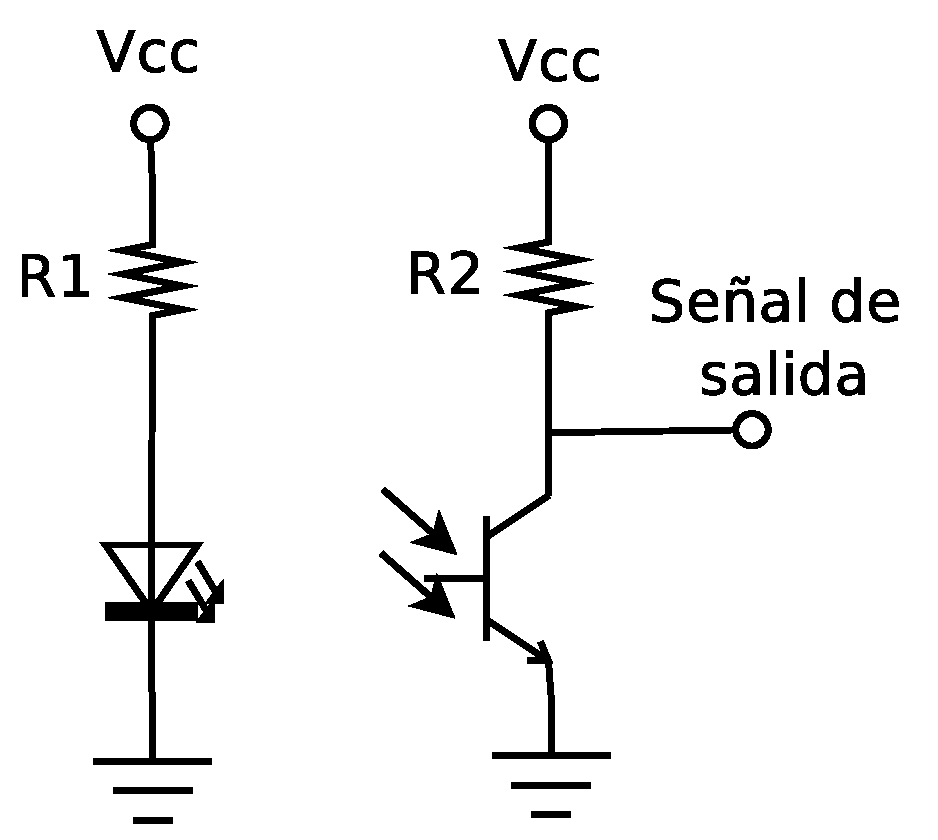
\includegraphics[width=0.75\textwidth]{Figures/Infrarrojo.eps}
    \caption{Circuito emisor-receptor IR.}
    \label{fig:CircuitoIR}
  \end{subfigure}
  \qquad\qquad
  \begin{subfigure}[b]{0.4\textwidth}
    \centering
    \includegraphics[width=0.75\textwidth]{Figures/SensorPoses.png}
    \caption{Posición de los sensores en el robot.}
    \label{fig:SensorPoses}
  \end{subfigure}
\caption{Sensores de distancia.}
\end{figure}

La tarjeta Arduino Uno sólo tiene seis convertidores analógico-digitales, de los cuales dos están conectados a los mismos pines utilizados para la comunicación I2C, por lo que sólo quedan cuatro disponibles. Por esta razón, aunque la señal de salida del circuito IR es analógica, ésta se conectará a los pines lógicos de entrada del Arduino Uno. 

De acuerdo con la hoja de especificaciones del microcontrolador ATMega328P (el que utiliza la tarjeta Arduino Uno), cuando éste se alimenta con $\textrm{V}_{cc}=5.0\textrm{V}$, el voltaje máximo para que una señal sea considerada como un cero lógico es de $0.3\textrm{V}_{cc}$, es decir, 1.5V, y el mínimo para detectar un uno lógico es de $0.6\textrm{V}_{cc}$, es decir, 3.0V. 

Por lo anterior, las resistencias R1 y R2 deben seleccionarse de modo que la señal de salida esté por debajo de 1.5V cuando haya un obstáculo ``cerca'', y por encima de 3.0V cuando el obstáculo esté ``lejos''. Los criterios para cerca y lejos no están fijos pero deben ser suficientes para que el robot pueda evadir obstáculos. Una distancia de 1 a 5 centímetros es razonable para un objeto cercano. 

\subsection{Conexión de los sensores al Arduino Uno}
Conecte las señales de salida de los sensores SD0, SD1, SD2, SD3, SD4, SD5, SD6 y SD7 (ver figura \ref{fig:SensorPoses}) a los pines de entrada 2, 4, 7, 8, 10, 11, 12 y 13 de la tarjeta Arduino Uno, respectivamente. La razón para usar estos pines es que los demás, digitales y analógicos, serán usados para otros dispositivos, como se muestra en la tabla \ref{tab:PinUsage}.

\begin{table}
\centering
\begin{tabular}{rll}
\hline
Pin & Dispositivo conectado & Descripción\\
\hline
0 & Serial Rx  & Comunicación serial con la RaspberryPi\\
1 & Serial Tx  & Comunicación serial con la RaspberryPi\\
2 & Sensor SD0 & Sensor de distancia binario\\
3 & Motor MA1  & Señal PWM para control del motor izquierdo\\
4 & Sensor SD1 & Sensor de distancia binario\\
5 & Motor MA2  & Señal PWM para control del motor izquierdo\\
6 & Motor MB1  & Señal PWM para control del motor derecho\\
7 & Sensor SD2 & Sensor de distancia binario\\
8 & Sensor SD3 & Sensor de distancia binario\\
9 & Motor MB2  & Señal PWM para control del motor derecho\\
10& Sensor SD4 & Sensor de distancia binario\\
11& Sensor SD5 & Sensor de distancia binario\\
12& Sensor SD6 & Sensor de distancia binario\\
13& Sensor SD7 & Sensor de distancia binario\\
A0& Sensor SLL & Sensor de luz izquierdo\\
A1& Sensor SLR & Sensor de luz derecho\\
A2& Sensor SB  & Sensor de batería\\
A3& Sensor ST  & Sensor de temperatura\\
A4& I2C SCL    & Comunicación con el acelerómetro\\
A5& I2C SDA    & Comunicación con el acelerómetro\\
\hline
\end{tabular}
\caption{Uso de los pines de la tarjeta Arduino Uno}
\label{tab:PinUsage}
\end{table}

\subsection{Nodo que publica los valores de los sensores}
Implemente un nodo en la tarjeta Arduino Uno (siguiendo un procedimiento similar a la práctica 3) que publique un tópico de tipo \texttt{std\_msgs::Float32MultiArray} con el nombre \texttt{/minirobot/hardware/sensors} que contenga las lecturas de los sensores de distancia. El tamaño del arreglo de flotantes contenido en el mensaje \textbf{debe ser 15}. Recuerde que el tamaño del arreglo se especifica en la variable \texttt{data\_length} del mensaje a enviar. Es importante que \textbf{el tamaño del arreglo sea 15} para el correcto funcionamiento de la GUI donde se desplegarán los valores de los sensores. 

El arreglo de flotantes del mensaje a publicar debe contener las lecturas de los sensores en el siguiente orden:
\begin{verbatim}
  {SD0  SD1  SD2  SD3  SD4  SD5  SD6  SD7  0  0  0  0  0  0  0}
\end{verbatim}

Es decir, de los quince datos, los primeros ocho corresponden a los sensores de distancia (que sólo tendrán dos posibles valores, 0 ó 1) y los demas deben ser ceros (serán usados en prácticas posteriores para el resto de los sensores). Por ejemplo, si los sensores SD0, SD2 y SD3 detectan objetos cercanos y los demás no, el contenido del arreglo debería ser:
\begin{verbatim}
  {0  1  0  0  1  1  1  1  0  0  0  0  0  0  0}
\end{verbatim}

con lo que la GUI desplegaría algo como lo que se muestra en la figura \ref{fig:Example}. Para correr la GUI y visualizar los datos, en una nueva terminal, ejecute el comando

\begin{lstlisting}[language=bash]
$  rosrun mini_robot_gui mini_robot_gui_node
\end{lstlisting}

\begin{figure}
  \centering
  \includegraphics[width=0.7\textwidth]{Figures/SensorExample.png}
  \caption{Ejemplo de lectura de sensores. SD0, SD2 y SD3 detectan objetos cercanos.}
  \label{fig:Example}
\end{figure}

\section{Evaluación}

\begin{itemize}
\item La distancia a la que los sensores deben detectar un objeto como ``cercano'' debe ser de entre 1 y 5 centímetros.
\item El correcto funcionamiento de los sensores se verificará con la GUI.
\item Los sensores ya deben estar montados en la estructura del robot.
\item Se acercarán objetos arbitrarios a los sensores y la detección debe verse claramente en la GUI.
\item Todos los sensores deben tener salidas similares ante distancias similares. 
\end{itemize}

\end{document}

%%% Local Variables:
%%% mode: latex
%%% TeX-master: t
%%% End:
